\documentclass[10pt,conference,compsocconf]{IEEEtran}

\usepackage{hyperref}
\usepackage{graphicx}	% For figure environment
\usepackage{amsmath}

\begin{document}
\title{Do theoretical guarantees in convex optimization algorithms hold in real machine learning problems?}

\author{
  Yui Chi Hung\\
  \textit{SCIPER: 319733}
}

\maketitle

\begin{abstract}
  There are a lot of theoretical guarantees supporting different convex optimization algorithms. This project aims to verify whether these theoretical guarantees also hold in real machine learning problems. The machine learning problem picked in this project is a binary classification problem. Logistic regression is used as the algorithm, and different convex optimization algorithms are used to optimize the corresponding loss function (Binary Cross-Entropy loss, in short, BCE loss). The results generally show that the theoretical guarantees are also true in this binary classification problem. It is also observed that the theoretical bounds are relatively tighter bounds with increasing number of iterations performed.
\end{abstract}

\section{Introduction and Experimental Setup}

The BCE loss is a typical loss function used for logistic regression. The optimization problem for the logistic regression is a minimization of the BCE loss function. The following shows the problem:
\begin{multline}
\min_{w \in R^d} f(w) = \min_{w \in R^d} \  \frac{1}{n}\sum_{i=1}^n \big( -y^{(i)}\log(\sigma(w^T x^{(i)}))\\
-(1-y^{(i)})\log(1-\sigma(w^T x^{(i)})) \big)
\end{multline}
where $\sigma : R\rightarrow R$, $\sigma(z) := \frac{1}{1+e^{-z}}$ is the sigmoid function.
Here for any $i$, $1\le i\le n$, the vector $x^{(i)}\in R^d$ is the $i$-th data sample, and $y^{(i)}\in\{0,1\}$ is the corresponding label.\par

The gradient and the Hessian is computed as below:
\begin{multline}
\nabla f(w) = \frac{1}{n}\sum_{i=1}^n \big( y^{(i)}(-1+\sigma(w^T x^{(i)}))x^{(i)}\\
+(1-y^{(i)})\sigma(w^T x^{(i)})x^{(i)} \big) \\
\nabla^2 f(w) = \frac{1}{n}\sum_{i=1}^n \big( y^{(i)}\sigma(w^T x^{(i)})(1-\sigma(w^T x^{(i)}))x^{(i)}{x^{(i)}}^T\\
+(1-y^{(i)})\sigma(w^T x^{(i)})(1-\sigma(w^T x^{(i)}))x^{(i)}{x^{(i)}}^T \big)\\
= \frac{1}{n}\sum_{i=1}^n \sigma(w^T x^{(i)})(1-\sigma(w^T x^{(i)}))x^{(i)}{x^{(i)}}^T
\end{multline}
Notice the Hessian is a sum of symmetric positive semi-definite matrix, so it is a symmetric positive semi-definite matrix. Therefore, the BCE loss function is convex. Moreover, the largest eigenvalue of $\nabla^2 f(w)$ is upper bounded by the average of the largest eigenvalues of $\sigma(w^T x^{(i)})(1-\sigma(w^T x^{(i)}))x^{(i)}{x^{(i)}}^T$ (which is $\sigma(w^T x^{(i)})(1-\sigma(w^T x^{(i)}))||x^{(i)}||^2$). Also, $\sigma(w^T x^{(i)})(1-\sigma(w^T x^{(i)}))\leq\frac{1}{4}$. So $f(w)$ is $L$-smooth, with $L=\frac{1}{4n}\sum_{i=1}^n ||x^{(i)}||^2$. This $L$ doesn't imply that $f(w)$ is not $L'$-smooth for any $L'<L$. $L$ is just a guaranteed upper bound, but it is used in all of the convex optimization algorithms implemented.\par

The dataset used in this project is taken from the LibSVM datasets named "LIBSVM : a library for support vector machines. ACM Transactions on Intelligent Systems and Technology, 2:27:1--27:27, 2011" made by Chih-Chung Chang and Chih-Jen Lin. The raw dataset has target values being -1 or 1. To use logistic regression, it is necessary to convert the target values to either 0 or 1.\par

In this project, our main focus of verifying theoretical guarantees is about the relationship of the difference $f(w_T)-f(w^*)$ and the number of iterations performed, where $w^*$ is the global minimum of the loss function and $w_T$ is the weight vector obtained just after performing $T$ iterations. Four algorithms are being implemented in this project, with one of the algorithms (Stochastic Gradient Descent, also called SGD) not having a theoretical guarantee stated in the lecture notes for smooth convex functions. The remaining three algorithms have the following theoretical guarantees:
\begin{multline}
\text{Gradient Descent (GD): }f(w_T)-f(w^*)\leq\frac{L}{2T}\|w_0-w^*\|^2\\
\text{Accelerated GD: }f(y_T)-f(w^*)\leq\frac{2L}{T(T+1)}\|w_0-w^*\|^2\\
\text{Projected GD: }f(w_T)-f(w^*)\leq\frac{L}{2T}\|w_0-w^*\|^2
\end{multline}
According to these theoretical guarantees, the learning rate should be $\frac{1}{L}$. For SGD, the learning rate will be set to $\frac{1}{L}$, because it is anticipated that the result will be similar to the Gradient Descent algorithm in expectation. To minimize the effect of randomness when computing stochastic gradients, a batch size of 16 is used. It is expected that the result will be similar to the GD algorithm, but the running time would be greatly decreased due to a large decrease in the number of gradients computed.\par

As the data is taken from reality (i.e. non-constructed), it is hard to calculate the minimum value of the loss function. A posteriori to the results obtained, SGD is the best algorithm for optimizing this problem in terms of time measured by number of computed gradients. As a result, a SGD algorithm is being run on the problem for a relatively large number of iterations to do an estimation of the minimum value of the loss function ($f(w^*)$). This allows us to do an estimation on $f(w_T)-f(w^*)$ in the algorithms being used. To verify the theoretical guarantees, the first 100 iterations of each algorithm will be considered. In addition, for projected GD, the closed convex set will be a high-dimensional $L2$-ball with radius 2. This number is used after trying for different radii and is picked for a better visualization between the difference with the typical GD algorithm.

%The aim of writing a paper is to infect the mind of your reader with
%the brilliance of your idea~\cite{jones08}. 
%The hope is that after reading your
%paper, the audience will be convinced to try out your idea. In other
%words, it is the medium to transport the idea from your head to your
%reader's head. 
%In the following
%section, we show a common structure of scientific papers and briefly
%outline some tips for writing good papers in
%Section~\ref{sec:tips-writing}.

%\section{The Structure of a Paper}
%\label{sec:structure-paper}

%Scientific papers usually begin with the description of the problem,
%justifying why the problem is interesting. Most importantly, it argues
%that the problem is still unsolved, or that the current solutions are
%unsatisfactory. This leads to the main gist of the paper, which is
%``the idea''. The authors then show evidence, using derivations or
%experiments, that the idea works. Since science does not occur in a
%vacuum, a proper comparison to the current state of the art is often
%part of the results. Following these ideas, papers usually have the
%following structure:
%\begin{description}
%\item[Abstract] \ \\
  %Short description of the whole paper, to help the
  %reader decide whether to read it.
%\item[Introduction] \ \\
  %Describe your problem and state your
  %contributions.
%\item[Models and Methods] \ \\
  %Describe your idea and how it was implemented to solve
  %the problem. Survey the related work, giving credit where credit is
  %due.
%\item[Results] \ \\
  %Show evidence to support your claims made in the
  %introduction.
%\item[Discussion] \ \\
  %Discuss the strengths and weaknesses of your
  %approach, based on the results. Point out the implications of your
  %novel idea on the application concerned.
%\item[Summary] \ \\
  %Summarize your contributions in light of the new
  %results.
%\end{description}


\section{Results and evaluations}
This section will first provide graphs concerning each algorithm, then an analysis on the algorithms is provided at the end.
\subsection{GD algorithm}
A graph of $f(w_T)-f(w^*)$ versus the reciprocal of the iteration number is plotted. The axis are chosen from the theoretical guarantee saying that $f(w_T)-f(w^*)$ should be upper bounded by a multiple of $\frac{1}{T}$.
\begin{figure}[tbp]
  \centering
  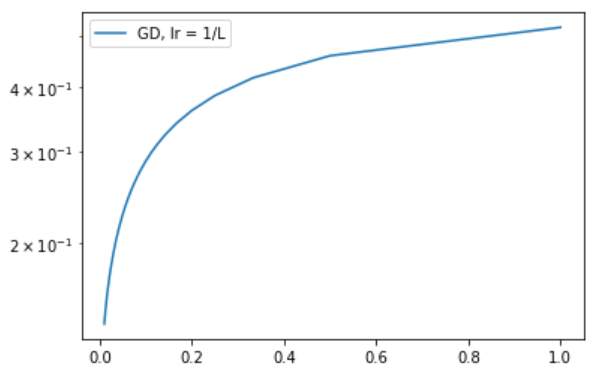
\includegraphics[width=\columnwidth]{gd}
  \caption{GD: $f(w_T)-f(w^*)$ versus $\frac{1}{T}$}
  \vspace{-3mm}
  \label{fig:gd}
\end{figure}

\subsection{Accelerated GD algorithm}
A graph of $f(y_T)-f(w^*)$ versus the square of the reciprocal of the iteration number is plotted. The axis are chosen from the theoretical guarantee saying that $f(y_T)-f(w^*)$ should be upper bounded by a multiple of $\frac{1}{T(T+1)}$.
\begin{figure}[tbp]
  \centering
  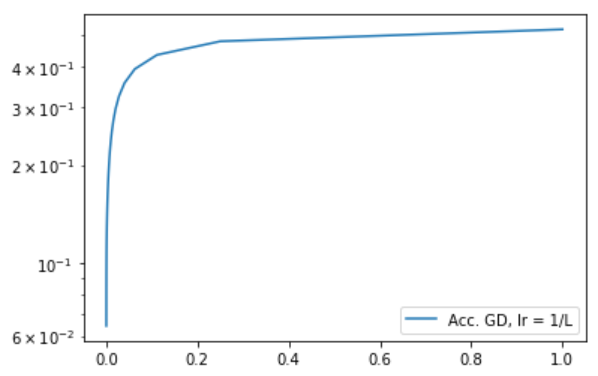
\includegraphics[width=\columnwidth]{accgd}
  \caption{Accelerated GD: $f(y_T)-f(w^*)$ versus $\frac{1}{T^2}$}
  \vspace{-3mm}
  \label{fig:accgd}
\end{figure}

\subsection{Projected GD algorithm}
A graph of $f(w_T)-f(w^*)$ versus the reciprocal of the iteration number is plotted. The axis are chosen from the theoretical guarantee saying that $f(w_T)-f(w^*)$ should be upper bounded by a multiple of $\frac{1}{T}$.
\begin{figure}[tbp]
  \centering
  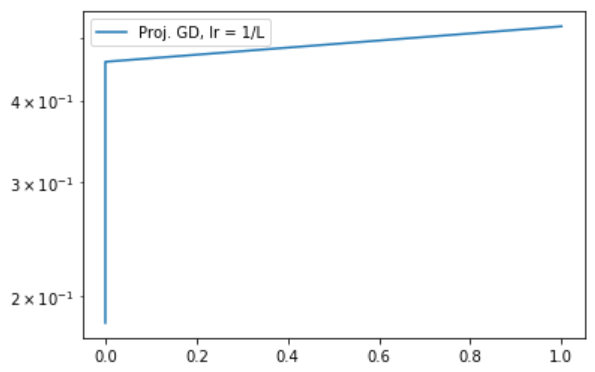
\includegraphics[width=\columnwidth]{projgd}
  \caption{Projected GD: $f(w_T)-f(w^*)$ versus $\frac{1}{T}$}
  \vspace{-3mm}
  \label{fig:projgd}
\end{figure}

\subsection{SGD algorithm}
A graph of $f(w_T)-f(w^*)$ versus the reciprocal of the iteration number is plotted. The axis are chosen from the guess that the result should be similar to the GD algorithm in expectation.
\begin{figure}[tbp]
  \centering
  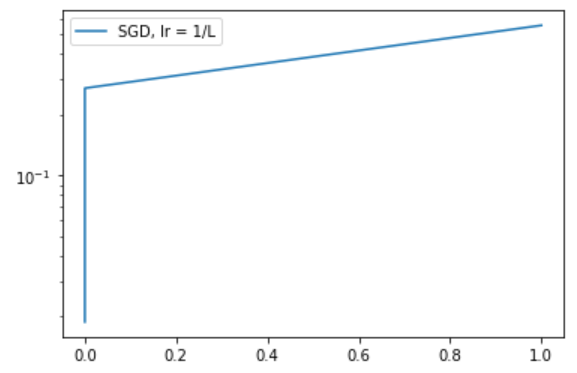
\includegraphics[width=\columnwidth]{sgd}
  \caption{SGD: $f(w_T)-f(w^*)$ versus $\frac{1}{T}$}
  \vspace{-3mm}
  \label{fig:sgd}
\end{figure}

\subsection{Analysis and perspectives}
For Fig.~\ref{fig:gd}, Fig.~\ref{fig:accgd}, Fig.~\ref{fig:projgd}, and Fig.~\ref{fig:sgd},  the slope of the graph at a point indicates $(f(w_T)-f(w^*))T$ (or $f(w_T)-f(w^*)T^2$ for accelerated GD), which shows whether the theoretical bound is tight. As the slope increases as the $x$-value becomes smaller, this means that the bound becomes tighter. Take $(f(w_T)-f(w^*))T$ in theoretical bound of GD algorithm as an example. $(f(w_T)-f(w^*))T\leq\frac{L}{2}\|w_0-w^*\|^2$, which means that a greater slope implies a closer value to the bound $\frac{L}{2}\|w_0-w^*\|^2$. This makes sense because $\frac{L}{2}\|w_0-w^*\|^2$ depends on $w_0$, which is decided prior to the iterated process. This allows the value varies a lot. Also, since all the graphs converges to 0 when $x$ goes to 0, this shows that all the theoretical bounds are in a correct order of convergence rate since $(f(w_T)-f(w^*))$ and $\frac{1}{T}$ (or $\frac{1}{T^2}$ for accelerated GD) are linear for large $T$, which verifies the correctness of the convex optimization algorithms in this real machine learning problem.\par
The following shows an overview comparison in terms of convergence speed and running time (in terms of number of computed gradients):\par
\begin{figure}[tbp]
  \centering
  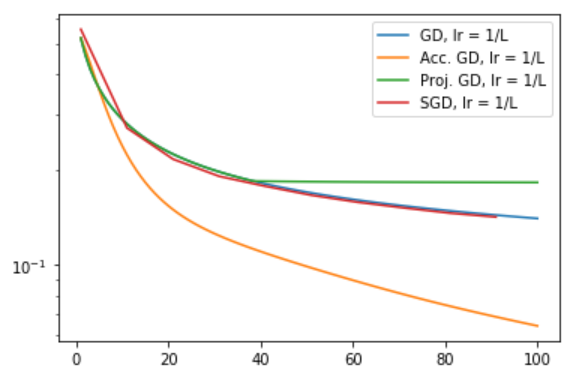
\includegraphics[width=\columnwidth]{compare_iter}
  \caption{Convergence speed: $f(w^T)$ versus $T$}
  \vspace{-3mm}
  \label{fig:compare_iter}
\end{figure}
\begin{figure}[tbp]
  \centering
  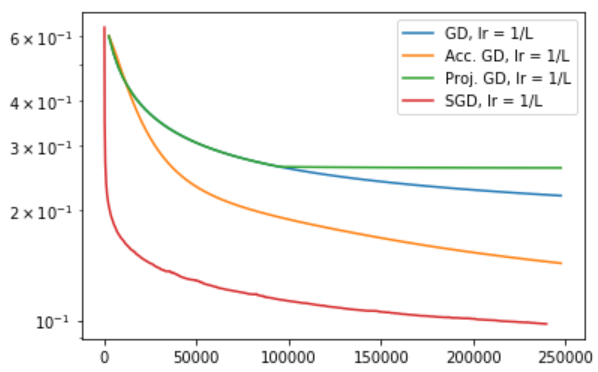
\includegraphics[width=\columnwidth]{compare_time}
  \caption{Running time: $f(w_T)$ versus no. of computed gradients}
  \vspace{-3mm}
  \label{fig:compare_time}
\end{figure}
Fig.~\ref{fig:compare_iter} shows that the accelerated GD algorithm has the fastest convergence rate, while the remaining algorithms have nearly the same convergence rate, which meets with the expectation and the theory. For the projected GD, it reaches a plateau at the middle since it is a constrained optimization problem, which restricts the norm of the iterated weight vector, hence resulting in an earlier convergence.\par
Fig.~\ref{fig:compare_time} shows that the SGD algorithm has the shortest running time, since it is the only algorithm not requiring to compute full gradients at each iteration. The small sacrifice of using a minibatch doesn't affect it to be a good algorithm for this problem. This may imply that SGD algorithm may also be useful for smooth convex functions despite not having a theoretical bound stated in the notes. Out of the remaining three algorithms, the accelerated GD algorithm has the shortest running time, which makes sense due to its fastest convergence rate.

\section{Summary}

The following are the conclusions from this project
\begin{itemize}
%\item Have a \texttt{README} file that (at least) describes what your
  %software does, and which commands to run to obtain results. Also
  %mention anything special that needs to be set up, such as
  %toolboxes\footnote{For those who are
  %particularly interested, other common structures can be found at
  %\url{http://en.wikipedia.org/wiki/README} and
  %\url{http://www.gnu.org/software/womb/gnits/}.}.
\item The theoretical bounds for GD algorithm, the accelerated GD algorithm, and the projected GD algorithm are all verified to be valid in this binary classification problem.
\item The bounds would be tighter with increasing number of iterations performed.
\item Although the lecture notes does not provide a theoretical bound for the SGD algorithm for smooth convex (but not necessarily strongly convex) functions, it has the best running time among all algorithms being implemented.
\end{itemize}

\section*{Acknowledgements and Resources}
The author thanks Chih-Chung Chang and Chih-Jen Lin for the dataset source, and the resources provided by Professor Martin Jaggi and Professor Nicolas Flammarion in the course CS-439 Optimization for machine learning under EPFL.\par
The libraries used in the Python codes are NumPy, SciPy, math, matplotlib, time, sklearn, and random.

%\newpage
%\bibliographystyle{IEEEtran}
%\bibliography{literature}

\end{document}
